

\section{Theory of operation}
\label{sec:Too}


\subsubsection{Master-Slave microcontroller configuration}

We use a pair of 32-bit microcontroller to capture and transmit data collected from the water meter.
The reason for this configuration stems from the fact that we were unable to completely switch off the GSM module on the
Arduino MKR GSM 1400 development kit (DK) which resulted in more energy consumption than we can meet with the off-grid solution
we have described in the last
section.
Thus, the master controls the infrared sensor, digitizes the sensor signal and accumulates a counter which it transmits to the
slave. The slave
transmits the data during selected time slots. The master controls power to the slave and the latter
is completely switched off outside of transmission intervals. We will discuss further details of the pro and cons of this configuration later in
this article.



\begin{figure}[h]
    \centering
    \begin{subfigure}[b]{0.45\textwidth}
        \centering
        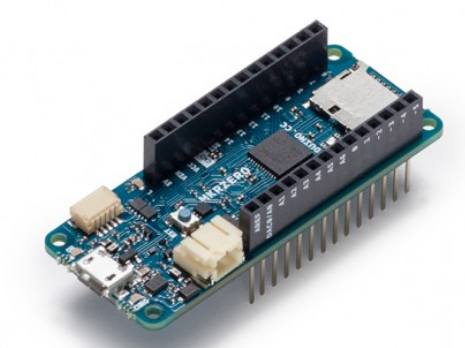
\includegraphics[width=.8\linewidth]{mkrzero}
        \subcaption{Master: Arduino MKR Zero DK}
        \label{fig:x}
    \end{subfigure}
    \hfill
    \begin{subfigure}[b]{0.45\textwidth}
        \centering
        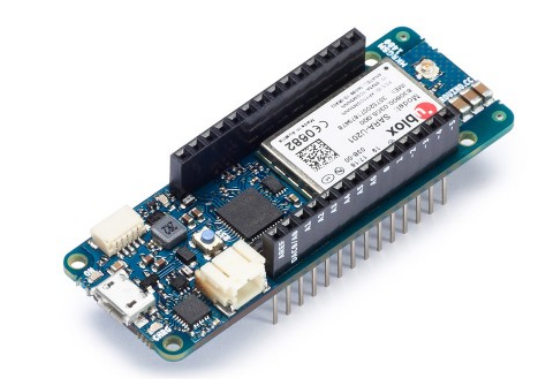
\includegraphics[width=.8\linewidth]{mkrgsm}
        \subcaption{Slave: Arduino MKR GMS 1400 DK}
        \label{fig:x}
    \end{subfigure}
    \caption{Master slave embedded system configuration}
    \label{fig:x}
\end{figure}
\subsubsection{Master-Slave handshake operation}

The master increments a counter on each high-low transition of the phototransistor's collector voltage.
This value is accumulated during 24 hours and then uploaded to a server that is accessible via the Internet.
Since the upload is done by the slave, the counter value must be transferred to the slave (via I2C).
Once this value has been successfully transferred, the slave sends a success code to the master and the counter
is updated with the number of increments that  occurred between the request to the slave and the reply from the slave.
\par

In case the data could not be transferred within in a given budget of attempts, the slave sends a failure code.
In either case the slave is shutdown by the master after the reply has been received.
In case of failure, the master will not reset the counter and start
another transmission attempt later.
The slave might also get stuck while attempting to transmit data. In this case, the slave firmware makes no progress and no
reply is sent to the master. To avoid a deadlock, the master will simply switch of the slave after a given delay and consider
the transmission attempt as failed.
\par
The transmission is done via the I2C bus.
Once the slave is powered on, it will connect its I2C interface with the one of the master controller via analog switches.
This allows data to be exchanged in both directions.
The analog switches provide I2C bus isolation. Since the slave controller can be powered of while the master controller is
powered on, the former would  be back-powered via the I2C IO pins through the internal
ESD diode. This situation can cause malfunctions and violates the Absolute Maximum Ratings of the SAMD21 microcontroller
hosted on the Arduino DKs.
This situation must therefore be avoided.


\section{Module structure}


In the following section, we present the embedded system hardware as a set of modules.
Modules can be composed of hardware components like resistors or integrated circuits (IC).
A module can also contain other modules in a nested, tree-like structure.

Modules are interconnected with nets. Nets are labeled, for example \textit{5V} or \textit{B}.
A net is labeled  in the module where it first occurs in a top-down manner. It can then been referred to
in a child module by prepending a dot to the label. For example, given that net \textit{\emph{B}} has been introduced
in the top-level module, it will be referred to as \textit{\emph{.B}} in any child module.
This notation is inspired from object-oriented programming.
A net has also an Id and a Rank. The former is a sequential number starting at 1 that is local to each module.
Rank is a hint on how important the net is when it comes to PCB layout. For example, nets carrying high-speed signals
or supply power are usually higher ranked than a net that controls a user LED.
